

\chapter{Research Environment}
\label{chapt::Subject}
The present chapter provides a discussion of the research context, the tools used, and the solutions implemented. 

The research environment is designed to train and evaluate reinforcement learning agents in selected Rummikub game tasks. It combines game mechanics implementation, an agent interface compatible with the ML-Agents Toolkit, a Curriculum Learning task generator and mechanisms for recording training results and evaluations. The environment supports the two methods under analysis: PPO Baseline and PPO\_GAIL. Rather than replicating the full human-computer game interface during training, its purpose is to provide controlled experimental conditions in which selected agent skills can be introduced and evaluated incrementally.

The research system consists of a game environment running in Unity, the ML-Agents trainer running on the Python side, YAML configuration files, describing the hyperparameters, a demonstration file used by PPO\_GAIL, and modules responsible for recording and analyzing results. The environment stores the current state of the game, generates a task that agent must complete, prepares observations, executes the agent’s actions, and awards rewards. The ML-Agents trainer uses the accumulated experience to update the shared policy.

The following versions of the tools were used as part of this project:
\begin{itemize}
	\item Unity 2022.3.48f1
	\item ML-Agents 0.30.0
	\item Python 3.9
	\item PyTorch 2.8.0 +cu128
\end{itemize}

\section{Game environment}

Rummikub was selected as the game environment due to its combination of simple rules and complex decision-making requirements. Although the basic objective of the game is easy to understand, achieving an effective strategy requires managing incomplete information, selecting beneficial actions from many possible combinations, and considering both current and future game states.

Rummikub is a challenging game for an artificial agent because the game state changes after every move. The agent must decide which tiles to play and how to arrange them on the board. It also needs to consider whether drawing additional tiles might be more advantageous than performing an action. The possibility of rearranging existing tile groups also introduces a large action space, making the game ideal for investigating reinforcement learning approaches.

The choice of Rummikub allows the evaluation of an RL agent in a setting that combines strategic planning, exploration of possible actions, and adaptation to changing conditions, while maintaining a well-defined rule system required for controlled experiments.



\subsection{Characteristics of the problem}
The main challenge in developing an artificial intelligence agent for Rummikub lies not in implementing the game rules, but in enabling the agent to make effective decisions in a complex, dynamic environment. At each turn, the agent must select an action based on the current game state, taking into account the possible future consequences of its decisions. Due to the combinatorial nature of Rummikub, a relatively simple set of rules can lead to a large number of possible states and actions.
From a reinforcement learning perspective, Rummikub can be represented as a sequential decision-making problem. The agent interacts with the environment by observing the current state, selecting an action and receiving feedback based on the outcome of the action performed. However, the game's characteristics, including a large state space, a variable action space, delayed rewards, and the necessity of long-term planning, make this problem challenging.

\subsection{Game Rules}
Rummikub is a board game where the main objective of the players is to get rid of all tiles in the rack. The game consists of 106 tiles, divided into eight sets of tiles in four colors ranging from 1 to 13, as well as two jokers which can be used to replace any other tile. The game involves two to four players, and it starts with each player receiving fourteen tiles. The game requires each player to put tiles on a 24-by-10 board, in predefined horizontal sequences:
\begin{itemize}
	\item group - contains 3 to 4 tiles, where each tile has the same value but different color,
	\item run - contains 3 to 13 tiles, where each tile is in the same color in ascending order.
\end{itemize}
In the first round, each player must place clear sequences on the board without utilising tiles from other sequences. The total value of these sequences must be at least 30 points. Points are assigned based on the numbers used to create the sequences and the joker takes on the value of the tile it replaces.

Once a player has reached their first turn and cannot place at least one tile, they must draw an extra tile from the bank.
The game ends when one player's rack is empty. Players' rankings are estimated based on the tiles remaining in their racks. If one of the players has a joker in their rack, it adds 30 points to their score. The lower the final score, the better.
The game also ends if one of the players must draw a tile from the empty bank. The final score is calculated in the same way, and the player with the fewest points wins \cite{rummikub_rules}.
 \subsection{Game implementation}
 As part of this work, a Rummikub game environment was implemented in the Unity engine, comprising the representation of the board and tiles, the rules of the game, the handling of moves, the user interface, a rule-based player, and a reinforcement learning agent. The environment was then integrated with the Unity ML-Agents Toolkit library, which facilitates communication between the Unity simulation and the training process running on the Python side, as well as the implementation of the PPO algorithm and the GAIL mechanism.
This was achieved by using components of the engine, which are divided into the following main modules:
 \begin{itemize}
 	\item The board game module, which consists of game map objects that can be interacted with. It includes grid objects, 3D tile prefabs, and interactions for moving or adding tiles.
 	\item  The user interface module is the part of the game that is visible to human players. It consists of text, buttons and game tiles. Players can see their own tiles, how many tiles other players have, how much time is left in their turn, and how many tiles are left in the bank.
 	\item A controller module that integrates the game's logic with its visual elements.
 	\item The game logic module, which includes validating the correctness of a move against the game rules.
 	\item A user module responsible for storing data on the tiles that a given human player possesses.
 	\item A computer player module that implements an NPC with predefined movements using a rule-based system. This computer player is used as an expert to create a \textit{.demo} file, which is used by the GAIL system.
 	\item A machine learning module that implements a computer player using machine learning algorithms. The functions of the \textbf{ML-Agents} framework were used for this purpose.  
 \end{itemize}
 During a turn, the player or computer-controlled agent selects an action through the appropriate control module. The controller translates the selected action into an operation on the board, such as placing, removing, or moving a tile. The game logic module then verifies whether the resulting board state satisfies the implemented Rummikub rules. The controller updates the visual representation and proceeds with or rejects the move depending on the validation result.
 
 \subsection{Game Mechanics and User Interactions in the Game Environment}
To enable the use of Rummikub as a test-bed for training an artificial intelligence agent, the game was implemented as a digital simulation.
In this thesis, Rummikub is implemented as a 3D board game using Unity engine, while the RL computer player is designed using Machine Learning Agents Toolkit, described in \ref{subchap: ML-Agents}
The implementation focuses not only on reproducing the original game mechanics but also on providing a structured environment in which an agent can observe the current game state, perform actions, and receive feedback based on the outcome of its decisions.
The environment was developed in Unity, where the game logic, board representation, player interactions, and artificial intelligence interface were implemented as separate components. The digital representation of the game allows the state of the board and players to be controlled and evaluated during the training process.

The basic element of the game is a tile, represented by its numerical value and color. Each tile object stores information required for identifying valid groups and sequences. While regular tiles have values ranging from one to thirteen and come in the colors red, blue, orange and black, jokers have a value of 30 and are purple or magenta.
As the representation of the players' racks there is used the List container, which is a flexible component for inserting, removing and sorting objects. 
The game board is represented by a two-and-a-half-dimensional grid consisting of 240 possible positions. The placed tiles are rendered in Unity engine, during gameplay only occupied places are stored in dictionary, where the value is the tile and the key is the position of the object.

The available interactions with the board for the player consist of:
\begin{itemize}
	\item putting tile on the board,
	\item moving tile from one position to another,
	\item removing tile from board,
	\item reverse all made actions, 
	\item draw a new tile,
	\item end the turn.
\end{itemize}
A player can only restore a tile from the board to their rack if it was placed in the same turn. If not, the player cannot perform this action. The action of ending the turn requires the player to place at least one tile properly on board, if the player cannot place any tile, they must take the action of drawing the tile, which automatically ends the current turn. The action of reversing all actions is intended to assist players who have made too many incorrect changes to the board. It reduces the time needed to fix the board, allowing the player to perform a valuable action before time runs out.

Sequence validation occurs when the player places or moves a tile on the board. Sequence length revision occurs after the end-turn action, providing information on whether each sequence on the board has at least three tiles. 

The agent's decision-making process involves not only the available actions presented, but also deciding where to place or move the tiles. From the agent's perspective, these are separate decisions that must be made together. Similarly, selecting a tile from the rack creates another decision.


%

%The research framework was designed to evaluate the influence of Generative Adversarial Imitation Learning (GAIL) on the training process of a reinforcement learning agent in the developed Curriculum Learning environment for the game of Rummikub. 



%\section{Tools and environment framework}
%This subsection presents the tools and framework used to build the simulation environment and the agent training environment as part of this thesis. The description covers both the Unity engine, which serves as the basis for implementing the game environment, and the ML-Agents Toolkit, which acts as a layer integrating the environment with reinforcement learning algorithms.


%\subsection{ML-Agents Toolkit}


%\section{Architecture of the game}

%\section{Research Environment}
%Opisać środowisko, jest wpisane zadanie,

%od strony badacza - grę oraz zaimplementowan CL , ewaluacja , plik yaml 
%opis środowiska nauki i opis środowiska ewaluacji/testu
%opis komend w cmd, 
%opis procesu konfiguracji, uruchomienie nauki oraz ewaluacja


%The environment's tasks have been organized within the Curriculum Learning framework, ranging from basic tile placement mechanisms to more complex situations that require taking into account multiple configurations on the board. The current curriculum level defines the initial state of the board, the contents of the agent's hand, the available playing area, and the conditions for an episode's success. A detailed description of the levels is presented in the table \ref{tab:CL_seg}.

%The algorithm’s hyperparameters, neural network settings, reward signals, maximum number of steps, and Curriculum Learning parameters are defined in a YAML configuration file. The configurations used for PPO Baseline and PPO+GAIL are described in section~\ref{chpt3::confAndHyper}. For PPO+GAIL, the file also contains imitation signal parameters and the path to a prepared expert demonstration file.

\section{Agent training}
\label{Enhancement_tech_3}
This subsection presents the tools and framework used to build the simulation environment and the agent training environment as part of this thesis. The description covers 
%both the Unity engine, which serves as the basis for implementing the game environment, and 
the ML-Agents Toolkit, which acts as a layer integrating the environment with reinforcement learning algorithms.


ML-Agents does not provide a ready-made implementation of an agent capable of making moves in the game of Rummikub. The policy returns only numerical values corresponding to individual branches of the discrete action space. Therefore, as part of this work, it was necessary to define, independently, the observations passed to the neural network, the structure of the action space, the method for interpreting the model’s decisions, masks for unavailable actions, the reward function, and the conditions for starting and ending an episode. These functionalities were consolidated into an agent class inheriting from the \textit{Agent} class provided by ML-Agents.
%\subsubsection{ML-Agents training framework}
\label{subchap: ML-Agents}
The Machine Learning Agents Toolkit (ML-Agents) is an open-source framework engineered by \textit{Unity Technologies}. ML-Agents provides a standardized, actively maintained framework that connects the Unity simulation environment directly to a PyTorch backend. 
ML-Agents allows intelligent agents to be trained through interaction with highly complex environments, eliminating the need for the time-consuming manual implementation of reward allocation protocols and network communication. It is important to note that the ML-Agents library is architecturally bound to the Unity ecosystem and cannot be utilized natively inside any other game engine.

%\subsubsection{Architecture of the framework}
%podanie odróżnienia części co znajduje się w unity a co w python, jak wygląda komunikacja między obiema częściami

%\cite{juliani2020}
\subsection{Behavior parameters and agent setup}
The important part of training the agent using ML-Agents is proper configuration of the agent in the Unity engine. \textit{Behavior parameters} are responsible for setting up the input and output variables that are transferred from Unity to the neural network in the Python environment. The image \ref{fig:Agents_setup in unity} presents crucial variables \cite{unitymlagents40}:
\begin{itemize}
	\item The Behavior Name is an important name tag to apply a certain configuration file.
	\item Vector Observation is responsible for determining the number of observations sent to the neural network. This amount must be exactly as defined in the agent's script. The Stacked Vector sub-variable creates a containerized  version, whereby one action will send the current observation and a predefined number of previous observations.
	\item Actions define the output space of the agent, there are two types of action: continuous and discrete. Continuous actions enable an agent to select real-valued outputs from a specified range, resulting in an effectively infinite number of possible values. This type of action is particularly well-suited to tasks that require precise control, such as determining the direction, speed or rotation of movement. In contrast, discrete actions enable the agent to select one option from a finite set of predefined values. For instance, a discrete branch of size two enables the agent to select either action 0 or action 1. This type is appropriate for selecting an object index or choosing between predefined actions, such as placing, moving, or removing a game element. An agent can perform more than one action in one move, known as \textit{branches}, which can be either continuous or discrete.  
	\item Model is a space to which a trained model can be attached. If left as \textit{None}, the environment will automatically be set to train. 
	\item Behavior Type defines the source of the action. There are three types. The first is the \textbf{Default}, where the decision is made by the NN from Python. \textbf{Heuristic}, where the user or expert maps the actions. \textbf{Inference} type uses a ready-made NN model in an \textit{.onnx} file.
\end{itemize}

\begin{figure}[h]
	\centering
	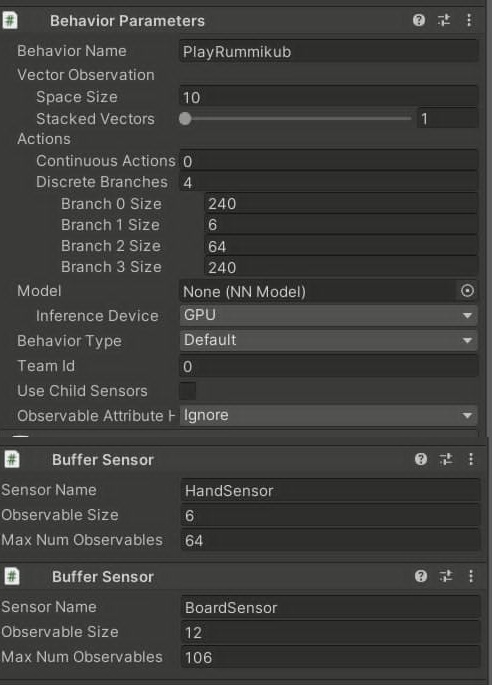
\includegraphics[width=0.7\textwidth]{images/BF_image.jpg}
	\caption{The image of behavior parameters of the agent in the Unity}
	\label{fig:Agents_setup in unity}
\end{figure}

Vector Observations are values that change over successive time steps, but the number of these variables remains constant. While it is possible to define volatile objects in Vector Observations, this creates unnecessary noise for the NN. In situations where the number of observations in the environment is volatile, the \textbf{Buffer Sensor} works best. This buffer serves as a flexible container that uses attention mechanisms to aggregate information for the NN. \cite{unitymlagents40}

There are crucial functions within the script that must be overridden: 
\begin{itemize}
	\item OnEpisodeBegin is function that is called at beginning of the episode during the simulation.
	\item CollectObservations is function called at beginning of every action of the agent. It is responsible to collect all observations that then are transfered to the NN.
	\item OnActionReceived is called after the NN analized the input from \textit{CollectObservations} function.
\end{itemize} 

% WriteDiscreteActionMask actionMask.SetActionEnabled 
% Heuristic
% Initialize
% AddReward SetReward
% EndEpisode


%Within the configuration file ML-Agents provides two methods belonging to \textbf{intrinsic motivation} mechanisms, \textbf{Intrinsic Curiosity Module} and \textbf{Random Network Distillation}. Although they are structurally built differently, their objective remains identical, which is to encourage agents to explore their environment more.


\subsection{Configurations and hyperparameters} 
\label{chpt3::confAndHyper}
Within the Python environment, NN has its predetermined, adjustable configurations that govern the fundamental behavior, training trajectory, and stability of a learning algorithm. They are positioned in a \textit{YAML} file, which is a human-readable data serialization language. 
YAML file organizes training variables in a nested hierarchical structure. \textit{hyperparameters, network\_settings, trainer configurations, behavioral\_cloning, reward\_signals and gail}. 

The YAML configuration file organizes training variables in a nested hierarchical structure. At the root of this hierarchy lies the specific behavior name, which contains high-level trainer configurations, such as defining the trainer type and maximum step count. Nested beneath this level are specialized sub-sections, including \textit{hyperparameters, network\_settings, reward\_signals}, and optional imitation learning modules like \textit{behavioral\_cloning} or \textit{gail}.
\cite{unitymlagentsTrainingConf}

\begin{lstlisting}[caption={Trainer Configuration Parameters.}, label={ls:YAML_trainerConf}]
	trainer_type: ppo
	max_steps: 5.0e5
	time_horizon: 64
	summary_freq: 10000
	checkpoint_interval: 50000
	keep_checkpoints: 5
	even_checkpoints: false
	threaded: false
	init_path: null
	hyperparameters:
	batch_size: 1024
	buffer_size: 10240
	learning_rate: 3.0e-4
	learning_rate_schedule: linear
\end{lstlisting}
Listening \ref{ls:YAML_trainerConf} presents exemplary configuration parameters. In this section there are chosen neutral variables that are common for each agent:
\begin{itemize}
	\item \textit{trainer\_type} defines type of learning algorithm. Provided trainers are ppo, sac and poca \cite{cohen2022}.
	\item \textit{max\_steps} is the maximal amount of steps collected in the environment during training process. 
	\item \textit{time\_horizon} is the amount of steps required to collect before appending it to the experience buffer.
	\item \textit{summary\_freq} defines the quantity of experience necessary to collect before summerisation and generation of the training statistics.
	\item \textit{checkpoint\_interval} is the number of experiences before saving the checkpoint. It serves as rescue in the event of critical error or malfunction of the device, thereby losing the progress.
	\item \textit{keep\_checkpoints} is the value of the most recent checkpoints stored in the device .
	\item \textit{even\_checkpoints} ignores \textit{checkpoint\_interval} and distributes the checkpoints equally  throughout the training simulation based on \textit{max\_steps} and \textit{keep\_checkpoints} settings, if it is set \textbf{true}.
	\item \textit{threaded} allows the environment to continue training while updating the model's weights.
	\item \textit{init\_path} defines the path to the previously trained model in order to continue learning.
	\item \textit{hyperparameters} defines predetermined, adjustable configurations that govern the fundamental behavior, training trajectory, and stability of a learning algorithm. The hyperparameters common to both the PPO and SAC algorithms are as follows:
	\begin{itemize}
		\item \textit{batch\_size} is the amount of steps in each iteration of gradient descent, it must be multiple times smaller than \textit{buffer\_size}.
		\item \textit{buffer\_size} defines the amount of steps to collect before updating the model's policy. 
		\item \textit{learning\_rate} defines starting learning rate for gradient descent
		\item \textit{learning\_rate\_schedule} determines the schedule of adjustment of \textit{learning\_rate} during training simulation. Can be set to \textbf{linear} or \textbf{constant}.
	\end{itemize}
\end{itemize}

\begin{lstlisting}[caption={Configuration of the neural network.}, label={ls:YAML_NN}]
	network_settings:
	vis_encode_type: simple
	normalize: false
	hidden_units: 128
	num_layers: 2
	memory:
	sequence_length: 64
	memory_size: 256
\end{lstlisting}
The listing \ref{ls:YAML_NN} display the example of the variables of the NN, which are common to all types of trainers:
\begin{itemize}
	\item \textit{vis\_encode\_type} defines the encoder type used for encoding visual observations
	\item \textit{normalize} applies the normalization process to the input values. 
	\item \textit{hidden\_units} defines the amount of artificial neurons in the hidden layer of the NN.
	\item \textit{num\_layers} defines the number of hidden layers in NN.
	\item \textit{memory} defines the memory enhancement for agent, which variables are as follows:
	\begin{itemize}
		\item \textit{sequence\_length} defines the length of the memory sequence of the experience that must be covered during the training simulation.
		\item \textit{memory\_size} is the size of the memory the agent must keep in its storage.
	\end{itemize}
\end{itemize}

\begin{lstlisting}[caption={PPO-specific hyperparameters.}, label={ls:YAML_PPO_hyperparameters}]
	hyperparameters:
	beta: 5.0e-3
	beta_schedule: constant
	epsilon: 0.2
	epsilon_schedule: linear
	lambd: 0.95
	num_epoch: 3
	shared_critic: False
\end{lstlisting}
The listing \ref{ls:YAML_PPO_hyperparameters} presents the example of hyperparameters specified for ppo trainer:

\begin{itemize}
	\item \textit{beta} variable defines entropy, which influences the stochasticity of the model's policy. The greater entropy, the more willing the agent is to take random actions.
	\item \textit{beta\_schedule} defines the decay schedule of beta variable.
	\item \textit{epsilon} affects the the rate at which the policy changes over time.
	\item \textit{epsilon\_schedule} is the decay schedule of epsilon variable
	\item \textit{lambd} defines the regularization variable $\Lambda$, which is used calculating the \textbf{Generalized Advantage Estimate} (GAE)
	\item \textit{num\_epoch} determines the amount of iteration through the experience buffer during gradient descent update.
	\item \textit{shared\_critic} is the boolean parameter that defines if actor-critic backbone is shared between Actor and Critic.
\end{itemize}
The \textit{poca} trainer shares the same specific configurations as the \textit{ppo} trainer.


\begin{lstlisting}[caption={Reward signals.}, label={ls:YAML_RS}]
	reward_signals:
	extrinsic:
	strength: 1.0
	gamma: 0.99
	
	gail:
	strength: 0.01
	gamma: 0.99
	demo_path: example/path/file.demo
	learning_rate: 3.0e-4
	use_actions: false
	use_vail: false
\end{lstlisting}
The reward signal configuration in listening \ref{ls:YAML_RS} presents the example of the setting parameters of both environment-based and GAIL reward signals. Each signal requires to implement at least two parameters, \textbf{strength} and \textbf{gamma}, also at least one reward signal should be implemented within configuration file.
\begin{itemize}
	\item \textit{extrinsic} defines the environment-based reward signals, which are configured within C\# script.
	\begin{itemize}
		\item \textit{strength} determines how much the reward signal influences the agent's behavior.
		\item \textit{gamma} influences the agent's prediction onto future rewards. Higher value determines that agent will seek for the long term rewards while smaller values determine the agent to seek the immediate rewards. 
		\item \textit{demo\_path} defines the location of the \textit{.demo} file.
	\end{itemize}
	
	\item \textit{gail} enables the module of \textbf{Generative Adversarial Imitation Learning} within configuration file. While it requires variables that repeat in previous configurations, it contains three individual parameters:
	\begin{itemize}
		\item \textit{use\_actions} determines if the discriminator penalizes the agent for both actions and observations or just for observations.
		\item \textit{use\_vail} creates a variational bottleneck in the GAIL discriminator, forcing it to learn a more general representation.
	\end{itemize}
	GAIL modul can also define its own network configuration, if it is not defined, it apples default settings of NN predefined by framework.
\end{itemize}

\begin{lstlisting}[caption={Example of curriculum learning configuration.}, label={ls:YAML_CL}]
	environment_parameters:
	my_environment_parameter:
	curriculum:
	- name: MyFirstLesson 
	completion_criteria:
	measure: progress
	behavior: my_behavior
	signal_smoothing: true
	min_lesson_length: 100
	threshold: 0.2
	value: 0.0
	- name: MySecondLesson 
	completion_criteria:
	measure: progress
	behavior: my_behavior
	signal_smoothing: true
	min_lesson_length: 100
	threshold: 0.6
	require_reset: true
	value:
	sampler_type: uniform
	sampler_parameters:
	min_value: 4.0
	max_value: 7.0
	- name: MyLastLesson
	value: 8.0
\end{lstlisting}
The listening \ref{ls:YAML_CL} presents exemplary configuration of \textit{curriculum learning} parameters.
\begin{itemize}
	\item \textit{- name} defines the identification tag, that is sent to the Unity environment.
	\item \textit{value} is defined by the user and sent to the Unity environment to be used within the script.
	\item \textit{completion\_criteria} is a parameter that must be implemented for the curriculum to be configured properly. It defines the conditions required for an agent to be promoted to a higher level.
	\begin{itemize}
		\item \textit{measure} defines how an agent's progress towards promotion is measured. Two main measurements can be implemented: reward, which identifies the minimum amount of reward required, and progress, which determines the ratio of steps/max\_steps expected to be completed before promotion.
		\item \textit{behavior} attach configured specifications to certain behavior due to the possibility of multiple different behaviors existing in one environment.
		\item \textit{threshold} determines the point value of measure that must be reached for a promotion.
		\item \textit{min\_lesson\_length} prevents the agent from being promoted too quickly due to the risk of failing to generalise the environment.
		\item \textit{signal\_smoothing} smooths the cumulative reward signal when the mean reward is measured. It prevents the agent from being promoted to a higher level due to unstable learning, whereby the agent receives a high reward spike instead of achieving consistently high performance. This setting is ignored in the case of a progress measure.
		\item \textit{require\_reset} determines whether or not the environment resets immediately after promotion.
	\end{itemize}
\end{itemize}
The configuration file contain more additional settings, such as SAC or self-play setting parameters, which can be found in \cite{unitymlagentsConfFile}.

To accelerate the training process, five independent instances of the Unity environment were executed in parallel using the \textit{--num-envs=5} parameter. Each instance simulated a separate game and collected experiences using the same agent policy. The observations, actions and rewards generated across all five environments were provided to a single training process and used to update the shared neural network. Furthermore, the environments were executed with the \textit{--no-graphics} option, which disabled graphical rendering and reduced the computational resources required by the Unity application. This configuration increased the rate at which training data were collected.

\subsection{Observation representation}
The agent receives a numerical representation of the current state of the game. The observations include the tiles on the board and those held by the agent, their values, colors and positions. The color of a tile is represented using \textit{one-hot} encoding, in which each available color corresponds to a separate position in the vector. The values of the tiles are normalized to the range from 0 to 1, so that their scale is adapted to the neural network’s input data. The position of a tile is represented by its coordinates in the board’s logical grid, which are also converted into a numerical form suitable for the model.

Observations prepared in this way do not directly contain Unity objects or visual information, they are merely numerical values. The state of the environment is transformed into an ordered set of values, on the basis of which the agent’s policy selects the next action.

%Since the board observations and rack observations are dynamical, for such containers there are implemented \textbf{Buffor Sensors}.

\subsection{Actions interpretation and masking}
%Another enhancement method implemented fundamentally by ML-Agents is \textbf{action masking}.

The agent’s action space has been defined as a multi-branch discrete space. The values returned by the model specify the type of action, the tile selected, and the source or target position on the board. The resulting numbers are interpreted by the agent class and converted into operations performed by the game logic, such as placing a tile, moving it, removing it, drawing a tile, undoing changes, or ending a turn.

The action branches of the agent goes as follows:
\begin{itemize}
	\item Target positions (0-239) - defines the final position of the tile, whether it is being put down or moved.  
	\item Function choice (0-5) - determines which interaction the agent will have with the board.
	\item Index choice (0-63) - Specifies the index of the tile from the list of tiles to be placed on the board. The range of values results from the maximum number of tiles that an agent can draw within the full game, assuming that opponents will not draw any tiles.
	\item Source position (0-239) - defines the source from where agent move tile or remove tile from the board
\end{itemize}

Since not all combinations of values correspond to actions available in a given game state, an \textit{action masking} mechanism has been implemented. Within the \textit{Agent} class, there is a \textbf{WriteDiscreteActionMask} method, that can disable certain values within branch. It is possible thanks to the \textit{SetActionEnabled(branch, actionIndex, isEnabled)} function, which requires the user to select a branch, a value within the chosen branch's range, and a flag. Masks prevent, among other things, the selection of a non-existent tile, an occupied position, or an action that is unavailable at a specific stage of the task. This allows the decision space to be restricted to moves that can be executed in the current state of the environment.

The agent used in the curriculum retains an action space designed with the full game in mind. This means that it also possesses actions that are not required at the levels currently being analyses, such as drawing or moving tile. Rather than creating a separate agent architecture for each task, unused actions are blocked using action masks. This allows subsequent levels of the curriculum to gradually introduce new mechanisms without altering the output structure of the neural network.

Since the board is stored in X-Z positioning, the source and target positions of the actions would be defined as four branches, meaning the agent would have to make four separate decisions to move a tile on the board. 
To reduce the number of decisions, \textbf{Matrix Index Mapping} was implemented, which translates 2D coordinates into a 1D linear vector. 

The mapping from 2D to 1D:
\begin{align}
	index = z \cdot xSize + x
\end{align}
Recovering the 1D vector as a 2D matrix:
\begin{align}
	\begin{cases}
		x = index\pmod{xSize} \\
		z = \left\lfloor \dfrac{index}{xSize} \right\rfloor
	\end{cases}
\end{align}
Where:
\begin{itemize}
	\item index presents single mapped board position,
	\item x and z are position coordinates,
	\item xSize defines the width of the board along the X-axis.
\end{itemize}
This technique allowed for the exclusion of illegal actions. If selecting a single position on the board required two separate action branches, for coordinates X and Z, standard action masking would not be feasible, as ML-Agents only supports masking actions independently within each individual branch

\subsection{Reward Function}
The foundational integrated method is \textbf{reward shaping}. The framework implements two methods: \textbf{SetReward}, which overwrites the currently accumulated reward with a specific input value, and \textbf{AddReward}, incrementally updates the total collected reward. Assigning a negative value to the function means it works as a penalty instead of a reward.

The reward mechanism implemented is not limited to awarding a reward for completing an episode or imposing a penalty for failure. The agent also receives an indirect signal for actions leading to the correct solution to the task. For example, if completing the task requires two moves, placing the first tile correctly may be rewarded regardless of the outcome of the next decision. If the second move is incorrect and the task is not completed, the agent will receive a final penalty, but its cumulative reward will be higher than if both actions had been incorrect. % This technique is called .

This approach makes it possible to distinguish between completely incorrect behavior and partial progress. The agent can thus gain insight into which actions bring it closer to the solution, even if the entire episode ends in failure. This is a form of \textit{reward shaping} function used to mitigate the problem of sparse rewards.

\subsection{Curriculum Learning Implementation}
The ML-Agents Toolkit provides a native implementation of curriculum learning, allowing to easily deploy this technique within the Unity environment. It requires a proper integration between the simulation scene and the training process. Within Python environment and configuration file, there must be defined the conditioning of transitioning between successive difficulty levels, like mean reward. Concurrently, within the Unity engine, a corresponding mechanism must be implemented to interpret the dynamic values sent from the training backend. This collaborative setup creates a seamless bridge that enables the complete automation of the learning process.

The curriculum levels have been implemented using a set of methods and flags that control the environment’s configuration. The ML-Agents trainer passes a parameter value to Unity that specifies the current curriculum level. Based on this, the environment selects the appropriate task variant, prepares the initial state of the board, assigns the required tiles to the agent, and activates the correct action masks and episode termination conditions.

Depending on the level, some tiles may be automatically placed on the board, whilst the remainder are assigned to the agent. The available area of the board, the number of moves, the type of required configuration and the set of permitted actions may also vary. This allows the same agent class to be used to complete tasks of progressively increasing difficulty.

Within the curriculum environment, no other players are involved in the tasks analyzed, and there is no turn-time limit. Removing these elements allows the learning process to focus on selected skills related to pattern recognition and tile placement. Despite these simplifications, the agent retains the observation and action structure designed with a view to its subsequent extension to the full game.

This thesis presents a Curriculum Learning \ref{an::CL} setting consisting of 12 levels of progress that introduce the agent to the Rimmikub game. A description of the stages is provided in the table \ref{tab:CL_seg}. 

\begin{longtable}{p{5cm} c p{8cm}}
	\caption{Stages of the implemented Curriculum Learning environment.}
	\label{tab:CL_seg}\\
	
	\toprule
	\textbf{Stage} &
	\textbf{Level} &
	\textbf{Main mechanisms} \\
	\midrule
	\endfirsthead
	
	\toprule
	\textbf{Stage} &
	\textbf{Level} &
	\textbf{Main mechanisms} \\
	\midrule
	\endhead
	
	\midrule
	\endfoot
	
	\bottomrule
	\endlastfoot
	Basic run placement & 0 & The agent observes two tiles belonging to a run set on the board. The agent's task is to correctly place the missing tile in the correct position. The sequence is assigned randomly at each episode. This tile can be the one on the right, left or middle. The agent has available only the first row of the board, which means 24 horizontal positions. The episode finishes when agent has no tiles in the ruck or the defined maximal amount of actions is reached.  \\
	\midrule
	Basic run placement & 1 & The task involves increasing the number of tiles that need to be put down. The agent observes one tile belonging to a run and must then place the remaining two tiles. \\ \midrule
	Basic run placement & 2 & The board is empty, the agent must place all three tiles in the correct positions to create a run.\\ \midrule
	Basic group placement & 3 & The task is the same as in task 0 but requires the agent to make proper group placement. \\ \midrule
	Basic group placement & 4 & The agent's task is to join two tiles from the same group to a tile that is already on the board. \\ \midrule
	Basic group placement & 5 & The agent must place a minimal group of three tiles on the board. \\ \midrule
	Mixed combinations & 6 & Agent receives scholastically three tiles of run or group and must place it properly on board.  \\  \midrule
	Mixed combinations & 7 & The amount of tiles increases to four tiles. \\  \midrule
	Mixed combinations & 8 & The amount of tiles is set to a range of between 3 and 4. \\  \midrule
	Mixed combinations & 9 & There are two sequences on the board: one is finished, while the other requires a tile to finish it. This task shows the agent that there can be more than one sequence on the board and that more tiles are not required. The unfinished sequence requires one tile from the agent.\\  \midrule
	Mixed combinations & 10 & The unfinished sequence requires two tiles from the agent. \\  \midrule
	Mixed combinations & 11 & On board there is one extra sequence on board, and the agent has to put one separate sequence on the board. \\  
\end{longtable}

\subsection{Demonstration recording}
At the configuration file, the ML-Agents framework also provides \textbf{imitation learning} method, \textbf{Generative Adversarial Imitation Learning}. Before integrating this method in configuration file, it is necessary to create demonstration recording of the \textit{expert}. It requires the method \textbf{Heuristic} to be overridden within the \textit{Agent} class and attachment of \textbf{Demonstration Recorder} to the agent's game object. The expert's recording can be generated through manual gameplay by a human operator or by predefined computer player algorithm, whose actions are mapped and configured into demonstration file. The \textit{.demo} file contains segregated sequences of observations, actions and rewards, through which the learning algorithm analyses the pairs state-action and adjusts the weights of NN to recreate actions in familiar situations. 

The demonstrations used by the GAIL mechanism were prepared using a rule-based computer player. This player acted as an expert, analysing the current state of the entire game and determining subsequent moves in accordance with the implemented rules.

The rule-based player’s decisions were passed to the agent class via a queue. This approach was adopted due to differences between the execution speed of the rule-based player’s logic and the decision-making cycle of the ML-Agents agent. The queue stored the prepared actions until the agent could retrieve them one by one and execute them in the environment.

Whilst recording the demonstration, the agent continued to generate observations of the environment and execute actions using the ML-Agents heuristic functions. The difference was that the action values did not come from a trained policy, but from decisions prepared by the rule-based algorithm. This made it possible to save observation–action pairs in the \textit{.demo} format required by the GAIL method.

The techniques described in this section represent the core methods used to support the training process in this project. Ml-Agents provides more auxiliary techniques, such as \textbf{intrinsic motivation} or \textbf{Behavior Cloning}. Additional training options provided by the toolkit are documented in detail in \cite{unitymlagentsOverview}.

\section{Communication Between the Game and Training Process}
ML-Agents operates as a highly integrated bridging architecture, connecting the C\#-based Unity game engine to external, Python-based deep learning frameworks. It deploys a specialized Python package that utilizes a \textit{gRPC} communication protocol paired with protocol buffer (protobuf) messages. This establishes a seamless, asynchronous data pipeline between the simulated environment and the optimization algorithms, allowing for accelerated training phases that can execute at speeds vastly exceeding real-time. However the actual training speed depends on the complexity of the unity environment and available device resources. 

\subsection{Architecture of the ML-Agents Framework}
Within the Unity engine, the internal software development kit (SDK) architecture is strictly partitioned into three fundamental hierarchical entities:
\begin{itemize}
	\item Sensors - these are utilized as observation extraction to as an integral part of MDP state space. Sensors are attached to agents and are explicitly responsible for collecting observational data. The architecture supports multimodal sensory inputs, meaning a single agent can simultaneously process continuous arbitrary length vectors, ray-cast collision detections, and high-dimensional rendered visual images.  
	\item Agents - the \textbf{Agent} component is fundamentally attached to a game object within the simulation, granting it the systemic capacity to gather observations from its sensors, execute distinct actions, and process environmental reward signals. A key feature of this architecture is the implementation of a \textbf{behavior name}, which identifies the underlying policy. The toolkit enables an unlimited number of agents within a scene to share the same behavior name. When grouped in such a manner, these agents synchronize their learning, executing the same policy and collectively pooling their trajectory experience data during the optimization phase. The architecture also enables policies to derive decisions from various distinct sources, such as hard-coded heuristic scripts, direct human input, embedded on-device neural networks or external Python API commands.
	\item Academy - It operates as a global singleton entity that manages the overarching logic of the simulation. Its primary functions are to track the discrete temporal steps of the simulation and to manage the lifecycle of all active agents. Additionally, the Academy handles \textit{environment parameters}, which are exposed variables that can dynamically alter the configuration of the simulated world at runtime. Through the Academy, an algorithm can manipulate gravity, re-scale objects, or adjust obstacle density dynamically, which constitutes the architectural backbone required for implementing advanced Curriculum Learning and Domain Randomization protocols.
\end{itemize}
\subsection{Training Data Flow}
On the external side of the architecture, the provided Python API initializes a \textbf{UnityEnvironment} class, which serves as the controller for launching and interfacing with the Unity executable. To maximize interoperability with the broader reinforcement learning research community, the toolkit architecture inherently provides wrapper APIs. These wrappers seamlessly convert the complex Unity communication pipeline into the standardized OpenAI Gym interface, permitting researchers to plug Unity environments directly into pre-existing reinforcement learning codebases without structural modifications.

The continuous execution loop that drives the training process between Unity and Python proceeds through the following computational steps:
\begin{enumerate}
	\item The \textbf{UnityEnvironment} class within the Python API initiates the connection to the Unity executable utilizing the gRPC protocol
	\item The internal Academy singleton configures the global environmental parameters (e.g. curriculum difficulty levels) for the upcoming episode.
	\item The Sensors attached to the in-game Agents collect the current environmental state data.
	\item The Agents package these observations, alongside any received rewards and terminal state flags, and transmit them through the Academy to the Python backend via serialized protobuf messages.
	\item The Python deep learning backend processes the incoming batch of experiences. Utilizing algorithms like PPO or SAC, it computes the objective functions and updates the neural network's mathematical weights.
	\item The Python API calculates the optimal next actions based on the updated policy and transmits this action vector back across the gRPC connection to the Unity environment.
	\item The Unity Agents receive the action vectors and execute the corresponding physical or logical movements. 
\end{enumerate}
The simulation progresses through the steps, and steps 2-7 repeat rapidly, until the policy converges to optimal behavior.

\section{Evaluation Metrics}
\label{Env::metrics}
During training process, the progress of each model was monitored using statistics recorded by TensorBoard, which is integrated with the ML-Agents framework by default. The data are stored in \textit{events.out.tfevents} event files. The analysis focused primarily on cumulative environmental reward, episode length and a custom curriculum-level statistic indicating when the agent was promoted to the next lesson. These metrics were selected because they directly reflected the agent's learning progress, the time spent on individual curriculum levels and any periods of stagnation or instability.

The analysis of every training run included whether the predefined target curriculum level had been reached within the established training budget, how many training interval steps had been required to reach this level and the corresponding wall-clock training time. The learning process was also examined in terms of stability. This was evaluated based on the variability of the environmental reward, the occurrence of extended stagnation periods and temporary decreases in performance during training. As all models were compared with respect to the same predefined target level, the highest curriculum level reached was not treated as a separate evaluation criterion.

Three principal metrics were selected to analyze the training process:

\begin{itemize}
	\item \textbf{Cumulative Reward} represents the sum of rewards and penalties received by the agent during an episode. Its increase generally indicates an improvement in the agent's behavior, although temporary decreases may occur after promotion to a more difficult curriculum level. Because the metric includes intermediate rewards and penalties, it should not be interpreted directly as the agent's win rate.
	
	\item \textbf{Environment/Lesson Number/level} is a metric recorded by ML-Agents in TensorBoard that indicates the curriculum lesson currently assigned to the agent. It allows training progression to be tracked and the approximate number of environment steps required to advance between successive tasks to be determined. Periods in which the value remains unchanged indicate how long the agent remained at a particular lesson before satisfying its promotion condition.
	
	\item \textbf{Policy Entropy} describes the randomness of the agent's policy and therefore the degree of exploration during training. Higher entropy indicates that actions are selected more randomly, whereas lower entropy indicates that the policy has become more deterministic.
	
\end{itemize}

Each evaluation episode was classified as either successful or unsuccessful. An episode was considered successful if the agent correctly completed the task defined for the selected curriculum level before the termination condition was met. Otherwise, the episode was classified as unsuccessful. The primary post-training metric was the success rate, calculated as follows:
\begin{equation}
	\text{Success Rate} = \frac{N_{\text{successful}}}{N_{\text{successful}} + N_{\text{unsuccessful}}}
\end{equation}
First, the success rate was calculated for each trained model separately. The results obtained by the ten models belonging to the same method were then aggregated to calculate the mean performance and variability between independent training runs. This procedure enabled comparison of the PPO baseline and PPO with GAIL not only in terms of their average effectiveness, but also in terms of consistency of results.
\subsection{Evaluation process}
The evaluation of the trained models is conducted directly within the simulated game environment implemented in the Unity engine. To this end, the exported \textit{ONNX} file is assigned to the component responsible for the agent’s behavior. Next, within the evaluation management object, the index of the agent being analyses, the number of episodes, the name of the resulting \textit{CSV} file and the curriculum level at which the test is to be carried out are specified.

The evaluation module allows the selection of any implemented curriculum level. It is not limited to level 11, which was used in the main experiments. This enables the model’s behavior to be examined both at the target level and on earlier tasks.

During evaluation, the model’s weights are not further updated. The agent uses only the policy stored in the \textit{ONNX} file, and mechanisms used solely during training, such as the additional GAIL signal, no longer influence the decisions made. Once the specified number of epi sodes has been completed, the module writes to a \textit{CSV} file, including, the agent’s index, the number of episodes played, the level on which it was evaluated on, the number of wins and losses, and the calculated win rate.

\section{Using the Research Environment}
In order to operate the trainer, it is necessary to establish a virtual Python environment with the ML-Agents package and other requisite dependencies installed:
	 \begin{verbatim}
	venv_3_9\Scripts\activate
\end{verbatim}
Then, after launching the environment, use the ML-Agents function:
\begin{verbatim}
	mlagents-learn ConfigurationFile.yaml --run-id=nameOfRun
\end{verbatim}
After a message appears indicating that the trainer is waiting for a connection, run the scene in the Unity editor by clicking the \textbf{Play} button. This option allows to observe how the environment works and was used primarily during implementation and troubleshooting.

More efficient way of the training is to activate many instances of the game, using the \textit{.exe} file of the game. The environment’s executable file is specified using the \texttt{--env} argument. Five independent instances of the game were launched simultaneously, and graphics rendering was disabled:
\begin{verbatim}
	mlagents-learn ConfigurationFile.yaml
	--run-id=nameOfRun
	--env=map\game.exe
	--num-envs=5
	--no-graphics
\end{verbatim}
Each instance generates separate episodes, but all instances are connected to the same policy. The collected observations, actions, and rewards are fed into a single training process, which used them to update a shared neural network.

The training process proceeded as follows:
\begin{enumerate}
	\item The ML-Agents trainer passes the current value of the \textit{curriculum} parameter to the Unity environment. Based on this value, the environment generated the appropriate board, the agent's hand, and the mission conditions.
	\item The agent collects observations describing the current state of the game, including information about the board, the stones in hand, and other game parameters. The observations were passed on to the policy running on the coach’s side.
	\item Before selecting an action, the game environment generates masks indicating actions that were unavailable in the current state. The policy then selected an action from among the permitted values of the individual branches of the discrete action space.
	\item The environment code interpreted the selected values as the type of action, the selected tile, and the source and target positions. Unity then carried out the action, updating the game state and awarding 
	\item Information about observations, actions, rewards and subsequent states are added to the set of experiences. Once the required number of experiences had been accumulated, the trainer used them to calculate the loss function and update the policy parameters.
	\item The episode continued until the task was completed, or a condition for defeat was met. Once the episode had ended, the environment saved its statistics and prepared a new initial state.
	\item The process was repeated until a defined target level or the maximum limit on training steps was reached.
\end{enumerate}
For each run, ML-Agents created a directory identified by the value \texttt{run-id}. This directory contained \textit{events.out.tfevents} event files, training checkpoints and the exported model in ONNX format. The event files contained standard ML-Agents metrics as well as custom environment statistics, including the current curriculum level, reward, episode length and promotion information. TensorBoard then enabled the visualisation of metrics such as cumulative environment reward, episode length and policy entropy. The ONNX model, meanwhile, contained the trained policy intended for deployment in Unity without any further parameter tuning.

The evaluation procedure utilized the exported ONNX model, which was assigned to the agent’s \textit{Behavior Parameters} component in the evaluation scene. The \textit{EvaluationManager} object specified the index of the agent under test, the number of episodes, the name of the output file, and the level at which the agent was to be evaluated. For each model, 1,000 episodes were run, during which wins and losses were counted. Once the evaluation was complete, the results were saved to a CSV file, including the agent’s index, the number of episodes played, the number of wins, the number of losses and the win rate.






%\section{Implementation}












%\subsubsection{Design of the agents}
%Funkcjonalność agenta w środowisku silnika wymaga odosobnionej implementacji. Framework ML-Agents dostarcza funkcji abstrakcyjnych, które muszą zostać zintegrowane z funkcjonalnościami gry. Sieć w python pozyskuje obserwacje z środowiska, po czym zwraca wartości zdefiniowane w \textit{Beharior Parameters}. 


%\subsubsection{Tensorboard}
% Tensorboard variables
%\section{Summary}
%\section{}
%\section{}





%\cite{rummikub_rules} source of rummikub rules

%\cite{unity_ml_agents_hyperparameters} source of hyperparameters information











%\chapter{[Subject of the thesis]}
%
%\begin{itemize}
%\item solution to the problem proposed by the author of the thesis
%\item theoretical analysis of proposed solutions
%\item rationale of applied methods, algorithms, and tools
%\end{itemize}
